\chapter{Discussion}
\label{chap:discussion}

The central result of this study is not that one algorithm ``solves'' material fire safety, but that the apparent predictive difficulty depends strongly on what is held out. When rows were divided at random, experiments from the same publication could occur in both training and test sets. Under that interpolation question, the flame-spread-rate (FSR) random-forest champion reached \(R^2=0.879\pm0.018\) with an RMSE of \(0.00626\pm0.00047~\mathrm{m\,s^{-1}}\), while the ignition XGBoost champion reached a ROC--AUC of \(0.908\pm0.010\). When complete papers were held out, the corresponding results fell to \(R^2=0.458\pm0.222\) and RMSE \(0.01221\pm0.00412~\mathrm{m\,s^{-1}}\) for FSR, and ROC--AUC \(0.718\pm0.044\) for ignition. The FSR error approximately doubled, and the ignition ROC--AUC decreased by about \(0.19\). This consistent row-versus-paper generalization collapse is the most consequential scientific finding. It indicates that models can interpolate effectively among conditions resembling a campaign already represented in training, but only partially transfer to an unseen publication, apparatus, laboratory practice, or sampled regime.

This chapter interprets that finding under four deliberately visible allocations: limitations, comparison with the literature, real-world applications, and future work. These reflect the practical importance of defining what the models do not establish and translating them into a cautious decision-support role.
\section{Limitations}
\label{sec:discussion_limitations}

\subsection{Threshold operating points}

The ignition classifier produces a probability, not an automatic fire-safety
decision. A deployed screening procedure must select a threshold at which a
predicted probability is converted into an ignition or no-ignition label. The
threshold policies considered in this work were selected from inner
out-of-fold predictions: maximum MCC, maximum F1, maximum balanced accuracy,
and maximum Youden's \(J\).

\Cref{fig:threshold-operating} shows the sensitivity--specificity trade-off
created by these policies. The interpolation champion provides useful operating
points within campaigns already represented in the database. However, the
paper-grouped extrapolation champion produces a much less reliable trade-off.
In particular, the F1 threshold strongly favours recall and can classify nearly
all observations from a new paper as ignition. This may be suitable for a
deliberately conservative initial alarm, but it is not a selective screening
rule.

The limitation is therefore not only that the model becomes less accurate on
unseen papers. It is that a threshold selected from known experimental sources
cannot yet be treated as a universal operating point for a new laboratory,
facility, campaign, or spacecraft configuration. Selecting a threshold remains
an explicit safety decision that must specify the relative cost of a missed
ignition and a false alarm.

\begin{figure}[htbp]
\centering

\includegraphics[width=0.5\textwidth]{threshold_operating_points.png}
\caption{Ignition operating points induced by the MCC, F1, and balanced-
accuracy/Youden-\(J\) threshold policies. Circles denote the interpolation
champion and triangles denote the paper-grouped extrapolation champion. F1
selects a low threshold and strongly reduces specificity under paper hold-out,
whereas MCC and balanced accuracy provide more balanced but still moderate
trade-offs on unseen papers.}
\label{fig:threshold-operating}
\end{figure}

\subsection{Rig fingerprints and ontology}

Rows from the same experimental campaign can share a rig, diagnostic method,
specimen preparation procedure, facility, flow system, atmosphere-control
method, and reporting convention. These factors can influence the observed
ignition and FSR outcomes even when they are not represented explicitly in the
current feature table. As a result, part of the difference between
interpolation and paper-grouped extrapolation may arise from experimental-rig
fingerprints rather than from the intended physical predictors alone.

A structured ontology is needed to separate physical conditions from the
experimental systems that produced the measurements. The ontology work we started
developping with Prof.~Guibaud and collaborators at ZARM in Bremen provides a
framework for representing experimental setup, sample properties, imposed
conditions, diagnostics, data reduction, and reported outcomes in a consistent
form. This is a parallel research activity, but it is directly relevant to the
present database: consistent rig and protocol metadata would make it possible
to identify comparable experiments, distinguish missing information from
inapplicable information, and eventually evaluate transfer across facilities
or rig classes.

\begin{figure}[htbp]
\centering
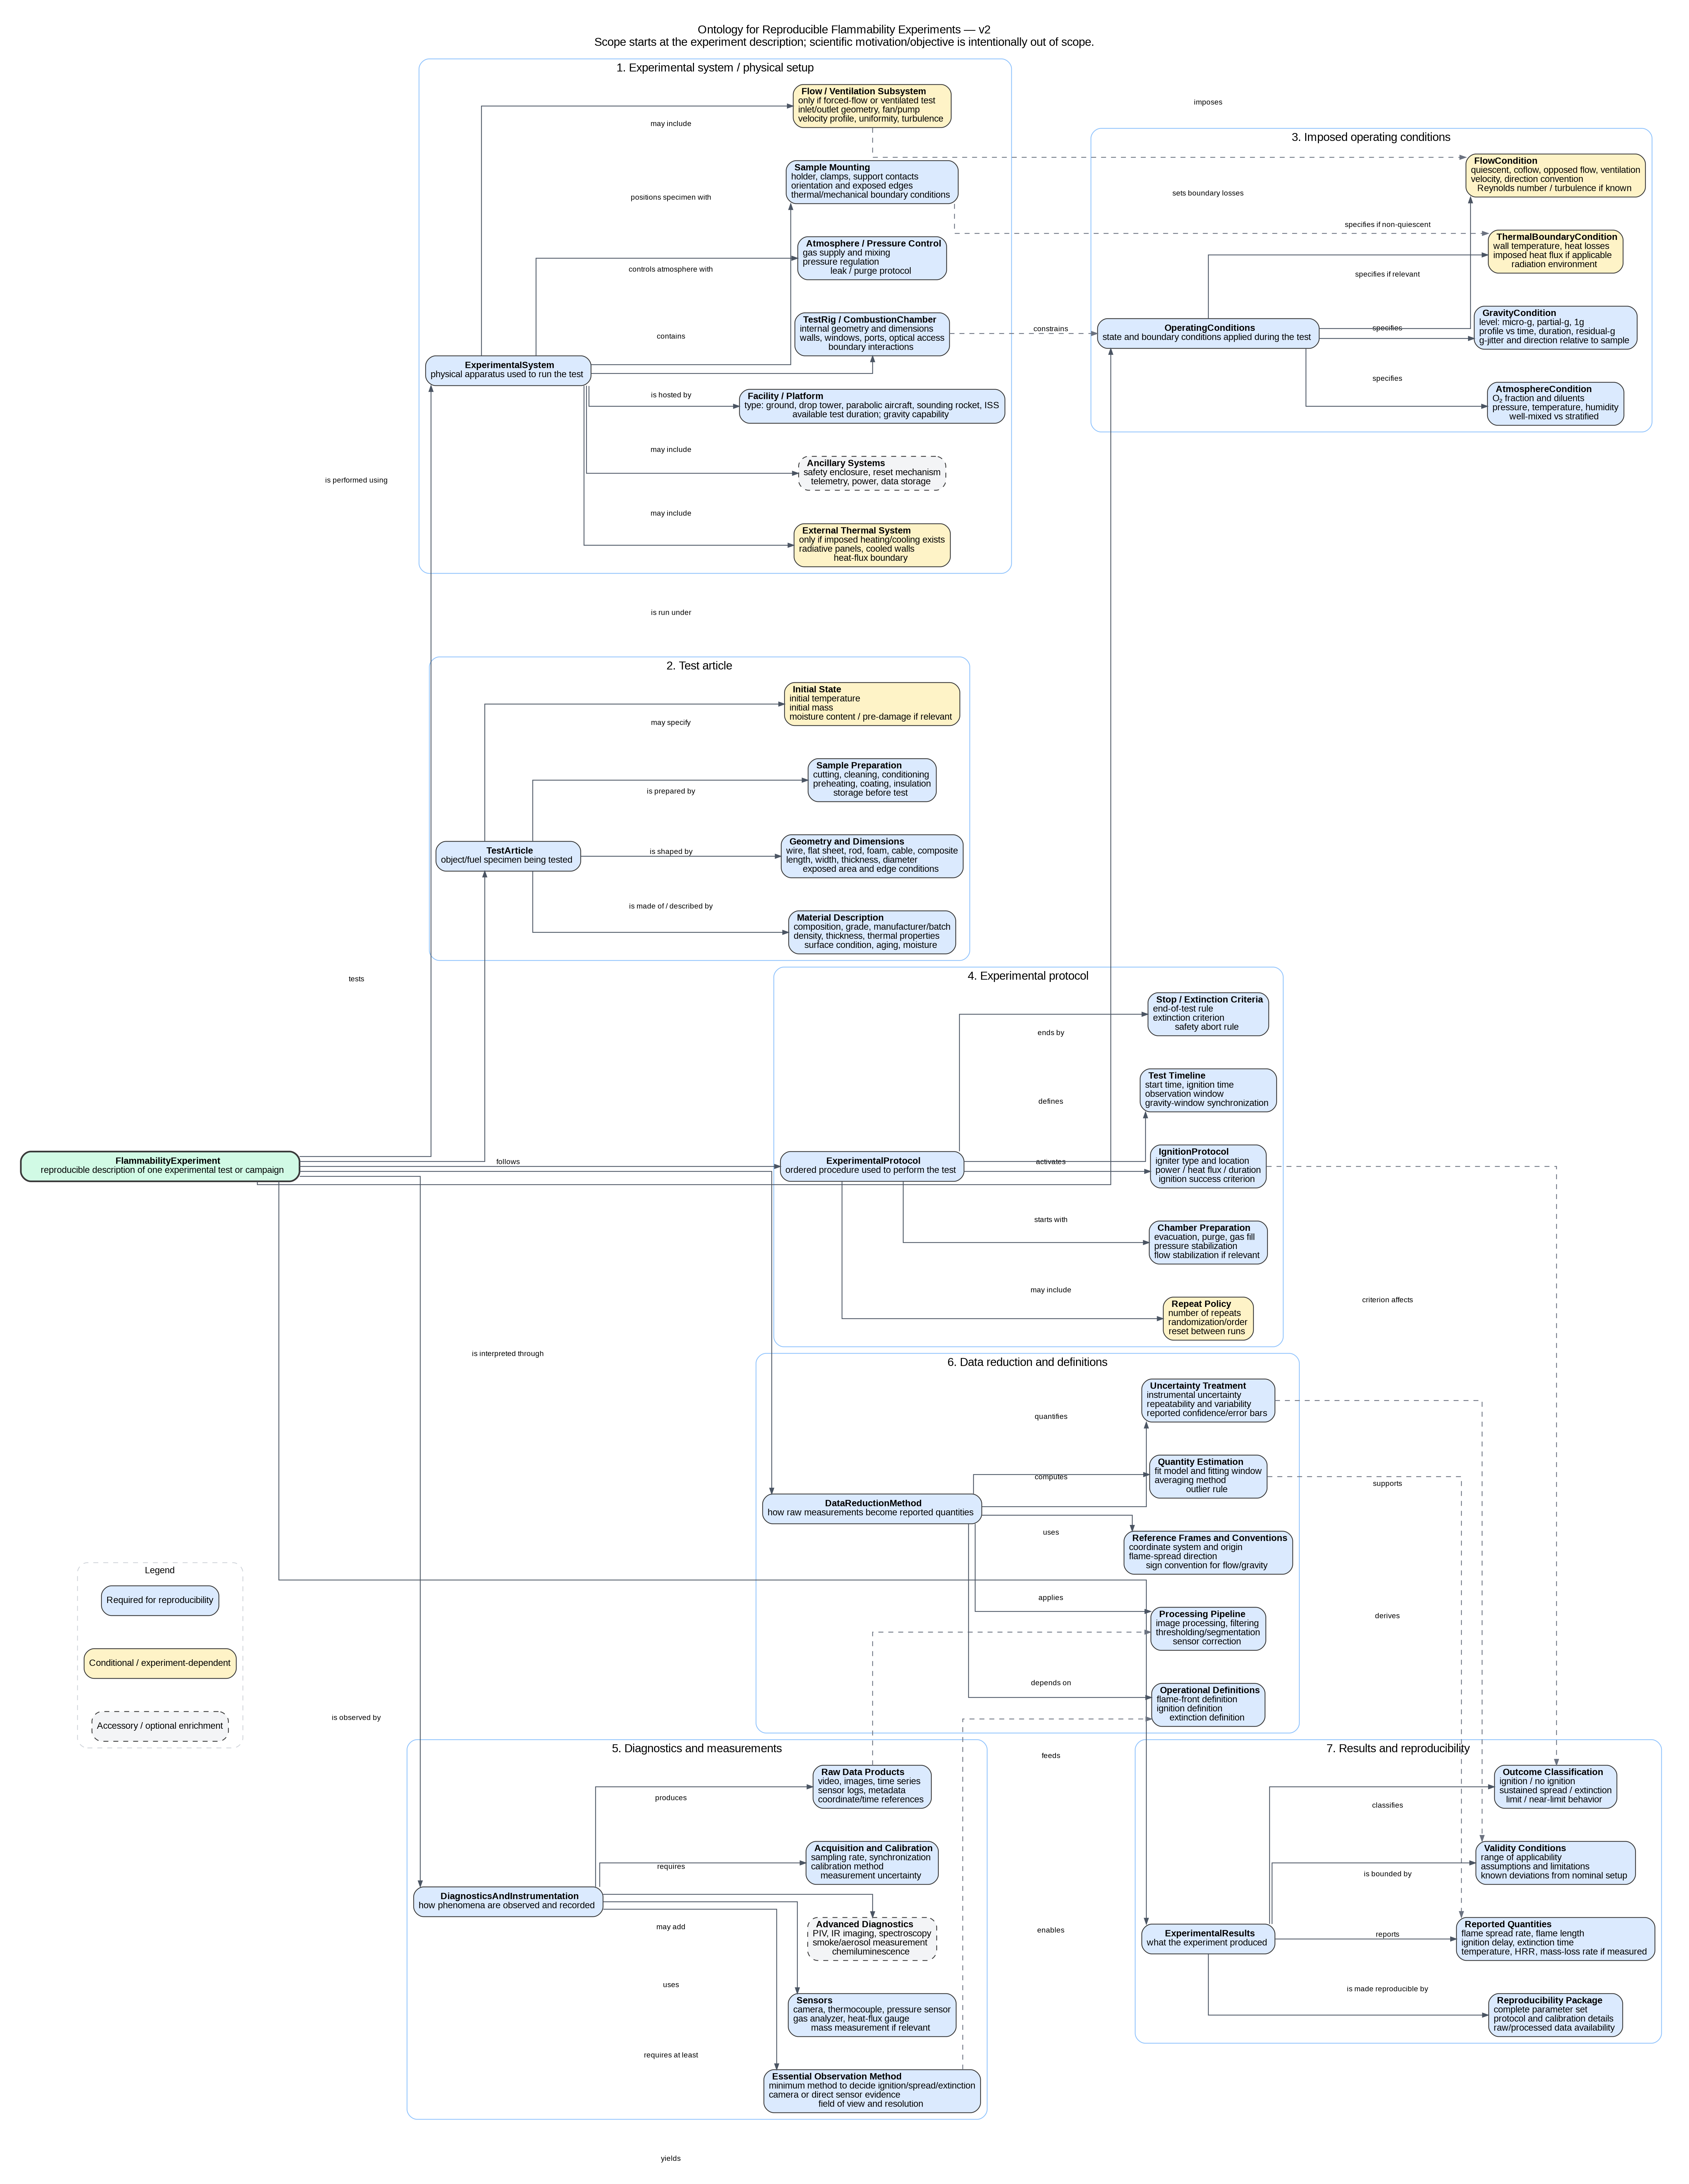
\includegraphics[width=0.7\textwidth]{figures/ontology.png}
\caption{Draft ontology for reproducible flammability experiments. The
structure separates the experimental system, test article, imposed operating
conditions, experimental protocol, diagnostics, data reduction, and reported
results. Zooming in is possible and encouraged.}
\label{fig:discussion-ontology}
\end{figure}

\section{Comparison with the Literature}
\label{sec:discussion_literature}

\subsection{Benchmarking against Rivera et al.}

Rivera, Jose, and colleagues compiled an approximately 1,200-observation
electrical-wire flame-spread dataset and evaluated several regression families
under random ten-fold cross-validation \cite{riveraWireML}. Their predictors
included wire-specific descriptors such as core material, insulation material,
spread direction, and configuration. They reported strong within-database
performance for nonlinear models, with several candidates exceeding
\(R^2=0.9\). Their target was reported in \si{\milli\metre\per\second}, and
their evaluation question was whether a model could predict another
observation from the compiled wire-data distribution.

The present study addresses a broader, more heterogeneous dataset containing
2,531 usable FSR observations from 66 canonical papers. It includes multiple
sample geometries, material systems, atmospheric conditions, gravity regimes,
and experimental facilities. FSR is standardised and evaluated in
\si{\metre\per\second}. The two studies therefore do not share the same
experimental population, target scale, feature representation, or evaluation
protocol.

The most important difference is the validation unit. Rivera et al.\ use random
cross-validation, which can place observations from the same experimental
source on both sides of a train--test split. Their reported \(R^2>0.9\) values
therefore quantify interpolation within the compiled wire database. The present
study reports both a comparable row-level interpolation result and a stricter
paper-grouped extrapolation result:

\begin{itemize}
  \item Under repeated row-level interpolation, the selected random-forest
  baseline reaches \(R^2=0.8790\pm0.0178\) and
  \(\mathrm{RMSE}=0.006263\pm0.000472~
  \si{\metre\per\second}\).

  \item Under paper-grouped extrapolation, where complete source papers are
  withheld, the same model reaches \(R^2=0.4576\pm0.2215\) and
  \(\mathrm{RMSE}=0.012205\pm0.004115~
  \si{\metre\per\second}\).
\end{itemize}

The interpolation result is the appropriate point of contact with
Rivera et al.'s random-cross-validation benchmark. It is somewhat lower than
their strongest wire-specific results, but the datasets remain too different
for a direct ranking of model quality. In contrast, the paper-grouped
\(R^2=0.458\) should not be described as being worse than Rivera et al.'s
\(R^2>0.9\), because Rivera et al.\ do not report an equivalent
source-held-out evaluation.

The combined evidence supports two conclusions. First, nonlinear tree-based
models are useful for flame-spread prediction in heterogeneous experimental
tables. Second, a high random-cross-validation score does not establish
transfer to an unseen publication, rig, or campaign. The difference between
the present interpolation and paper-grouped results makes the validation unit
part of the scientific claim rather than a technical detail.
```

\subsection{Tabular database findings}

XGBoost was the strongest ignition family under both interpolation and
paper-grouped extrapolation. This is consistent with its role as a strong
baseline for heterogeneous tabular data containing nonlinear interactions,
mixed feature types, unequal scales, and missing values.

For FSR, XGBoost remained competitive, but the random-forest baseline was
selected by the declared accuracy--stability policy. The result should not be
interpreted as a general claim that random forest is superior to XGBoost.
Rather, it shows that, within the evaluated candidate portfolio and frozen
splits, the random-forest baseline provided the preferred FSR trade-off.
Tree ensembles are therefore useful benchmark models for this database, but
their reported performance remains conditional on the represented experimental
sources and evaluation protocol.

\section{Real-World Applications}
\label{sec:discussion_applications}

The most immediate practical use of the database is to identify regions of the
experimental design space that remain poorly explored. \Cref{fig:o2-pressure-roadmap} maps observed ignition outcomes in oxygen--pressure space. It should
be interpreted as a coverage map rather than as a one-variable ignition
criterion: oxygen and pressure interact with fuel properties, geometry, flow,
gravity, and ignition conditions.

The dense sampling near terrestrial conditions does not imply that all nearby
spacecraft-relevant conditions are well represented. In particular, oxygen
concentrations just above the terrestrial value of approximately \(21\%\) and
pressures just below standard atmospheric pressure
(\(\approx 101~\si{\kilo\pascal}\)) are highly relevant to spacecraft
atmosphere design, yet are comparatively sparse in the assembled literature.
These conditions should be prioritised for new experiments, especially when
crossed with representative materials, flow conditions, geometries, and
gravity regimes.

The figure therefore provides a roadmap for targeted data collection. A model
may return a numerical prediction inside the marginal oxygen and pressure
ranges while the corresponding oxygen--pressure combination remains weakly
represented in the database. New experiments should preferentially fill such
sparse joint regions rather than add further repeats in already dense
terrestrial-pressure bands.

\begin{figure}[htbp]
\centering

\includegraphics[width=0.78\textwidth]{database_o2_pressure_ignition.png}
\caption{Observed ignition outcomes in oxygen--pressure space. The figure is
a roadmap for future experiments: regions with sparse observations, including
spacecraft-relevant conditions just above terrestrial oxygen concentration and
just below standard atmospheric pressure, require targeted measurements before
they can be treated as well-supported screening conditions.}
\label{fig:o2-pressure-roadmap}
\end{figure}

\newpage
\section{Future Work}
\label{sec:discussion_future}

The main next step for FSR regression is to introduce physical constraints.
The current models use physics-informed features, but the regression objective
does not yet require predictions to follow a flame-spread relation.

For counterflow, also called opposed flow, the imposed gas flow moves in the
direction opposite to flame propagation along the fuel. For concurrent flow,
also called co-flow, the imposed gas flow moves in the same direction as flame
propagation. These configurations have different heat-transfer and flame-spread
behaviour and should not be assumed to obey one common FSR relation.

For counterflow, the available physical description can distinguish thermally
thin and thermally thick materials. A thermally thin material has a temperature
field that can develop through most of its thickness during the relevant
heating and spreading time. A thermally thick material retains a substantial
internal temperature gradient and is governed by a different flame-spread
relation. The corresponding regime-specific counterflow equations can be used
to construct a physical loss: alongside the data-fitting error, the model can
be penalised when its predicted FSR is inconsistent with the applicable
thermally thin or thermally thick relation.

A central requirement is a reliable discriminator between the two thermal
regimes. The \texttt{thermal\_diffusion\_time} feature was introduced for this
purpose because it represents the time scale over which heat diffuses through
a characteristic material thickness. Future work should determine a
physically defensible regime boundary, validate it against experimental
conditions, and use it to apply the appropriate counterflow physical loss.

An equivalent reduced-order FSR relation is still needed for concurrent-flow
configurations. Deriving and validating such an equation would extend the
physical-loss approach beyond counterflow and would allow a future FSR model to
select a governing constraint using both flow direction and thermal regime.
Any resulting physics-constrained regressor should be evaluated with the same
paper-grouped protocol used in this study, so that improved physical
consistency is tested together with transfer to unseen experimental sources.